\documentclass[11pt]{article}
%\usepackage[14pt]{extsizes} % для того чтобы задать нестандартный 14-ый размер шрифта
%\usepackage[utf8]{inputenc}
\usepackage{mathtext}
\usepackage[english, russian]{babel}
\usepackage{amsmath}
\usepackage{amsfonts}
\usepackage{float}
\usepackage[margin=0.8in]{geometry}
\usepackage{multirow}
\usepackage{graphicx}
\usepackage[utf8x]{inputenc} % указать кодировку русского текста
\usepackage{fancyhdr}
\usepackage{indentfirst} % отступ в первой строке абзаца
\usepackage{wrapfig}
\usepackage{placeins}
\usepackage{wrapfig}
\usepackage{caption}
\usepackage{amssymb}
\usepackage{mathtools}
\usepackage[thinc]{esdiff}
%\usepackage{ upgreek }
\usepackage[table,xcdraw]{xcolor}
\pagestyle{fancy}
\begin{document}
\begin{titlepage}
\begin{center}
%\vspace*{1cm}
\large{\small ФЕДЕРАЛЬНОЕ ГОСУДАРСТВЕННОЕ АВТОНОМНОЕ ОБРАЗОВАТЕЛЬНОЕ\\ УЧРЕЖДЕНИЕ ВЫСШЕГО ОБРАЗОВАНИЯ\\ МОСКОВСКИЙ ФИЗИКО-ТЕХНИЧЕСКИЙ ИНСТИТУТ\\ (НАЦИОНАЛЬНЫЙ ИССЛЕДОВАТЕЛЬСКИЙ УНИВЕРСИТЕТ)\\ ФИЗТЕХ-ШКОЛА РАДИОТЕХНИКИ И КОМПЬЮТЕРНЫХ ТЕХНОЛОГИЙ}
\vfill
\line(1,0){430}\\[1mm]
\huge{Лабораторная работа 2.1.3}\\
\huge\textbf{Определение $\frac{C_p}{C_v}$ по скорости звука в газе}\\
\line(1,0){430}\\[1mm]
\vfill
\begin{flushright}
\normalsize{Устюжанина Мария}\\
\normalsize{\textbf{Группа Б01-107}}\\
\end{flushright}
\end{center}
\end{titlepage}
\fancyhead[L] {Работа 2.1.3}



\par \textbf{Цель работы:} 1) измерение частоты колебаний и длины волны при резонансе звуковых колебаний в газе, заполняющем трубу; 2) определение показателя адиабаты с помощью уравнения состояния идеального газа.

\par \textbf{В работе используются:} звуковой генератор ГЗ; электронный осциллограф ЭО; микрофон; телефон; раздвижная труба; теплоизолированная труба, обогреваемая водой из термостата; баллон со сжатым углекислым газом; газгольдер.

\section{Введение.}

В данной работе скорость звука измеряется 2мя способами, на двух установках(см рисунки). В обеих установках звуковые колебания в трубе возбуждаются телефоном Т и улавливаются микрофоном М. Мембрана телефона приводится в движение переменным током звуковой частоты; в качестве источника переменной ЭДС используется звуковой генератор ГЗ. Возникающий в микрофоне сигнал наблюдается на осциллографе ЭО.

Микрофон и телефон присоединены к установке через тонкие резиновые трубки. Такая связь достаточна для возбуждения и обнаружения звуковых колебаний в трубе и в то же время мало возмущает эти колебания: при расчетах оба торца трубы можно считать неподвижными, а влиянием соединительных отверстий пренебречь.

Первая установка (рис. \ref{img1}) содержит раздвижную трубу с миллиметровой шкалой. Через патрубок (на рисунке не показан) труба может наполняться воздухом или углекислым газом из газгольдера. На этой установке производятся измерения $ \gamma $ для воздуха и для $ CO_2 $. Вторая установка (рис. \ref{img2}) содержит теплоизолированную трубу постоянной длины. Воздух в трубе нагревается водой из термостата. Температура газа принимается равной температуре омывающей трубу воды. На этой установке измеряется зависимость скорости звука от температуры.

\begin{figure}[H]
\centering
\captionsetup{justification=centering}
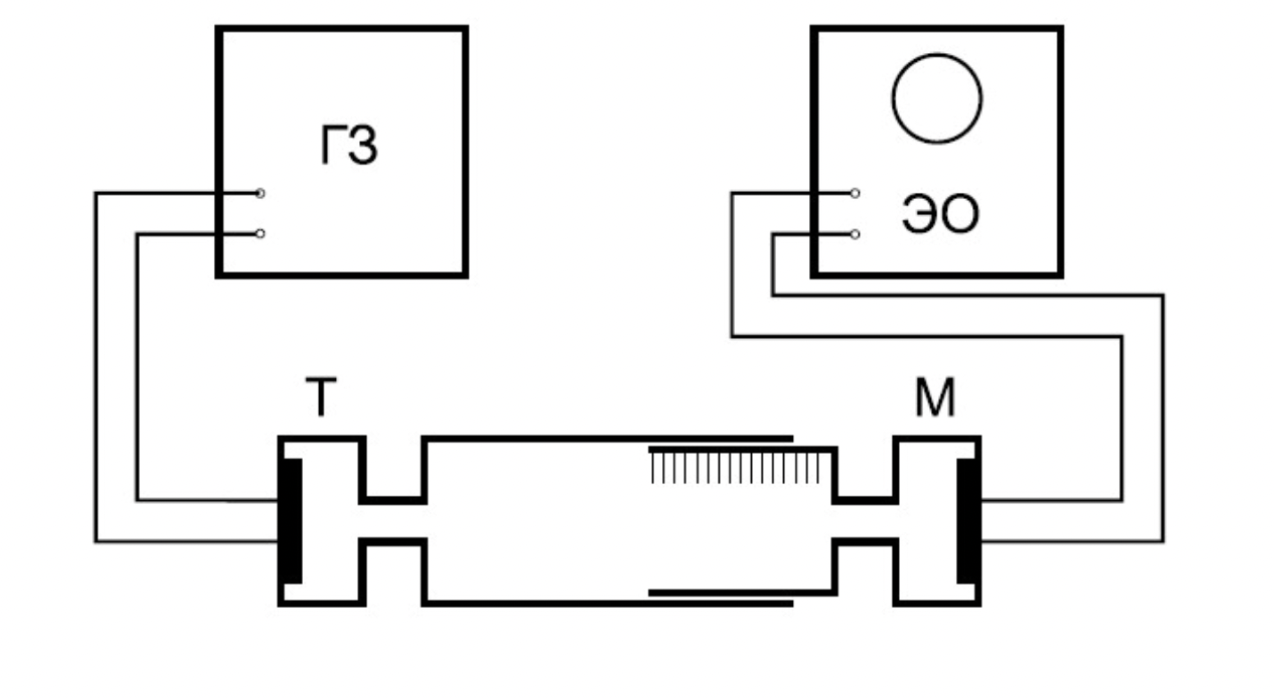
\includegraphics[width=0.5\textwidth]{Pic1.png}
\caption{Установка для измерения скорости звука при помощи раздвижной трубы.}
\end{figure}

\begin{figure}[H]
\centering
\captionsetup{justification=centering}
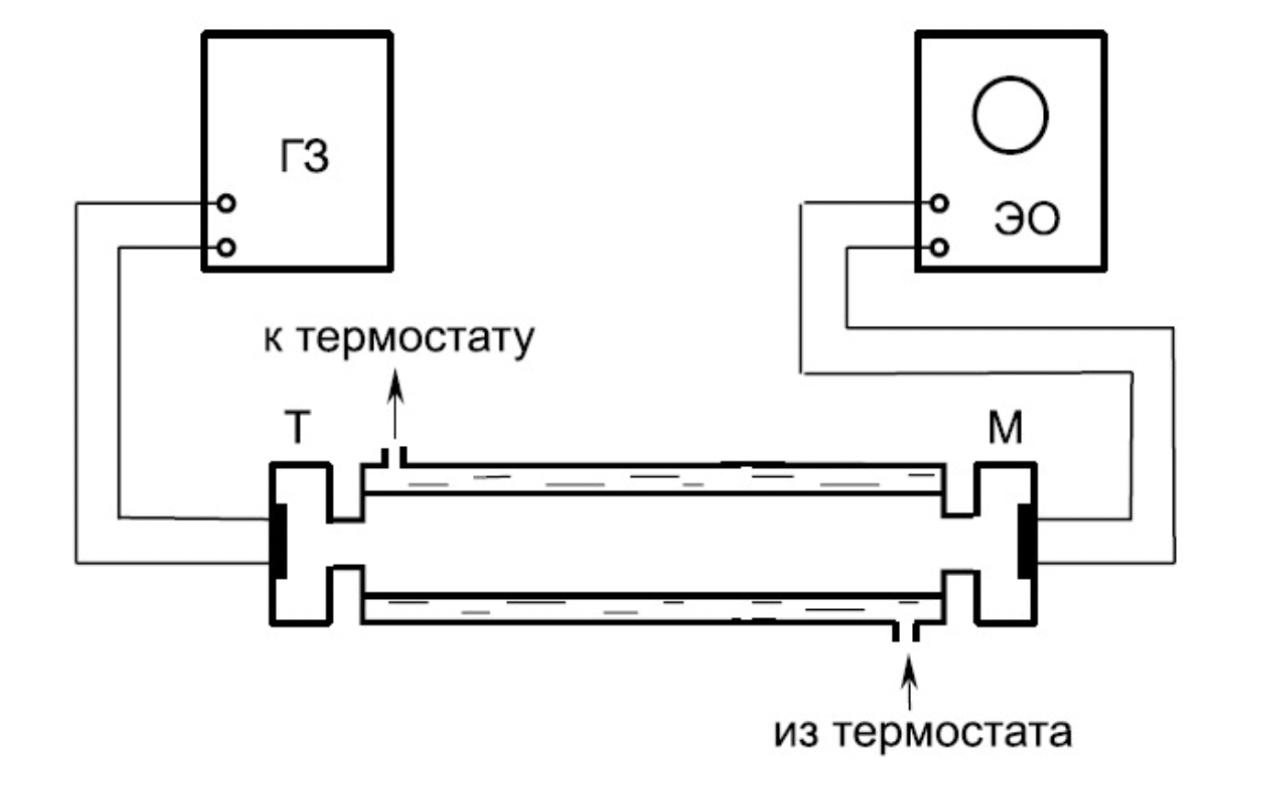
\includegraphics[width=0.25\textwidth]{Pic2.png}
\caption{Установка для изучения зависимости скорости звука от температуры.}
\end{figure}


\section{Обработка данных:}
\subsection{Измерение $ C_p/C_v $ для воздуха при помощи установки с раздвижной трубой}

Закачаем в первую установку воздух и будем плавно менять длину трубы, записывая значения длин, на которых будет наблюдаться резонанс.




    \begin{table}[H]
    \centering
    \caption{\textbf{Результаты измерений для воздуха}}
    \begin{tabular}{|r|r|r|r|r|}
    \hline
    \multicolumn{1}{|l|}{\textbf{Частота, кГц}} & \textit{3} & \textit{3,58} & \textit{4} & \textit{5} \\ \hline
    \textit{Удлинение 1, мм} & 0 & 0 & 0 & 0 \\ \hline
    \textit{Удлинение 2, мм} & 56 & 49 & 43 & 35 \\ \hline
    \textit{Удлинение 3, мм} & 113 & 97 & 85 & 69 \\ \hline
    \textit{Удлинение 4, мм} & \multicolumn{1}{l|}{-} & 145 & 128 & 106 \\ \hline
    \textit{Удлинение 5, мм} & \multicolumn{1}{l|}{-} & 193 & 171 & 138 \\ \hline
    \end{tabular}   
    \end{table}


    По полученным данным построим график:

    \begin{figure}[H]
    \centering
    \caption{График резонансов от удлинения трубы}
    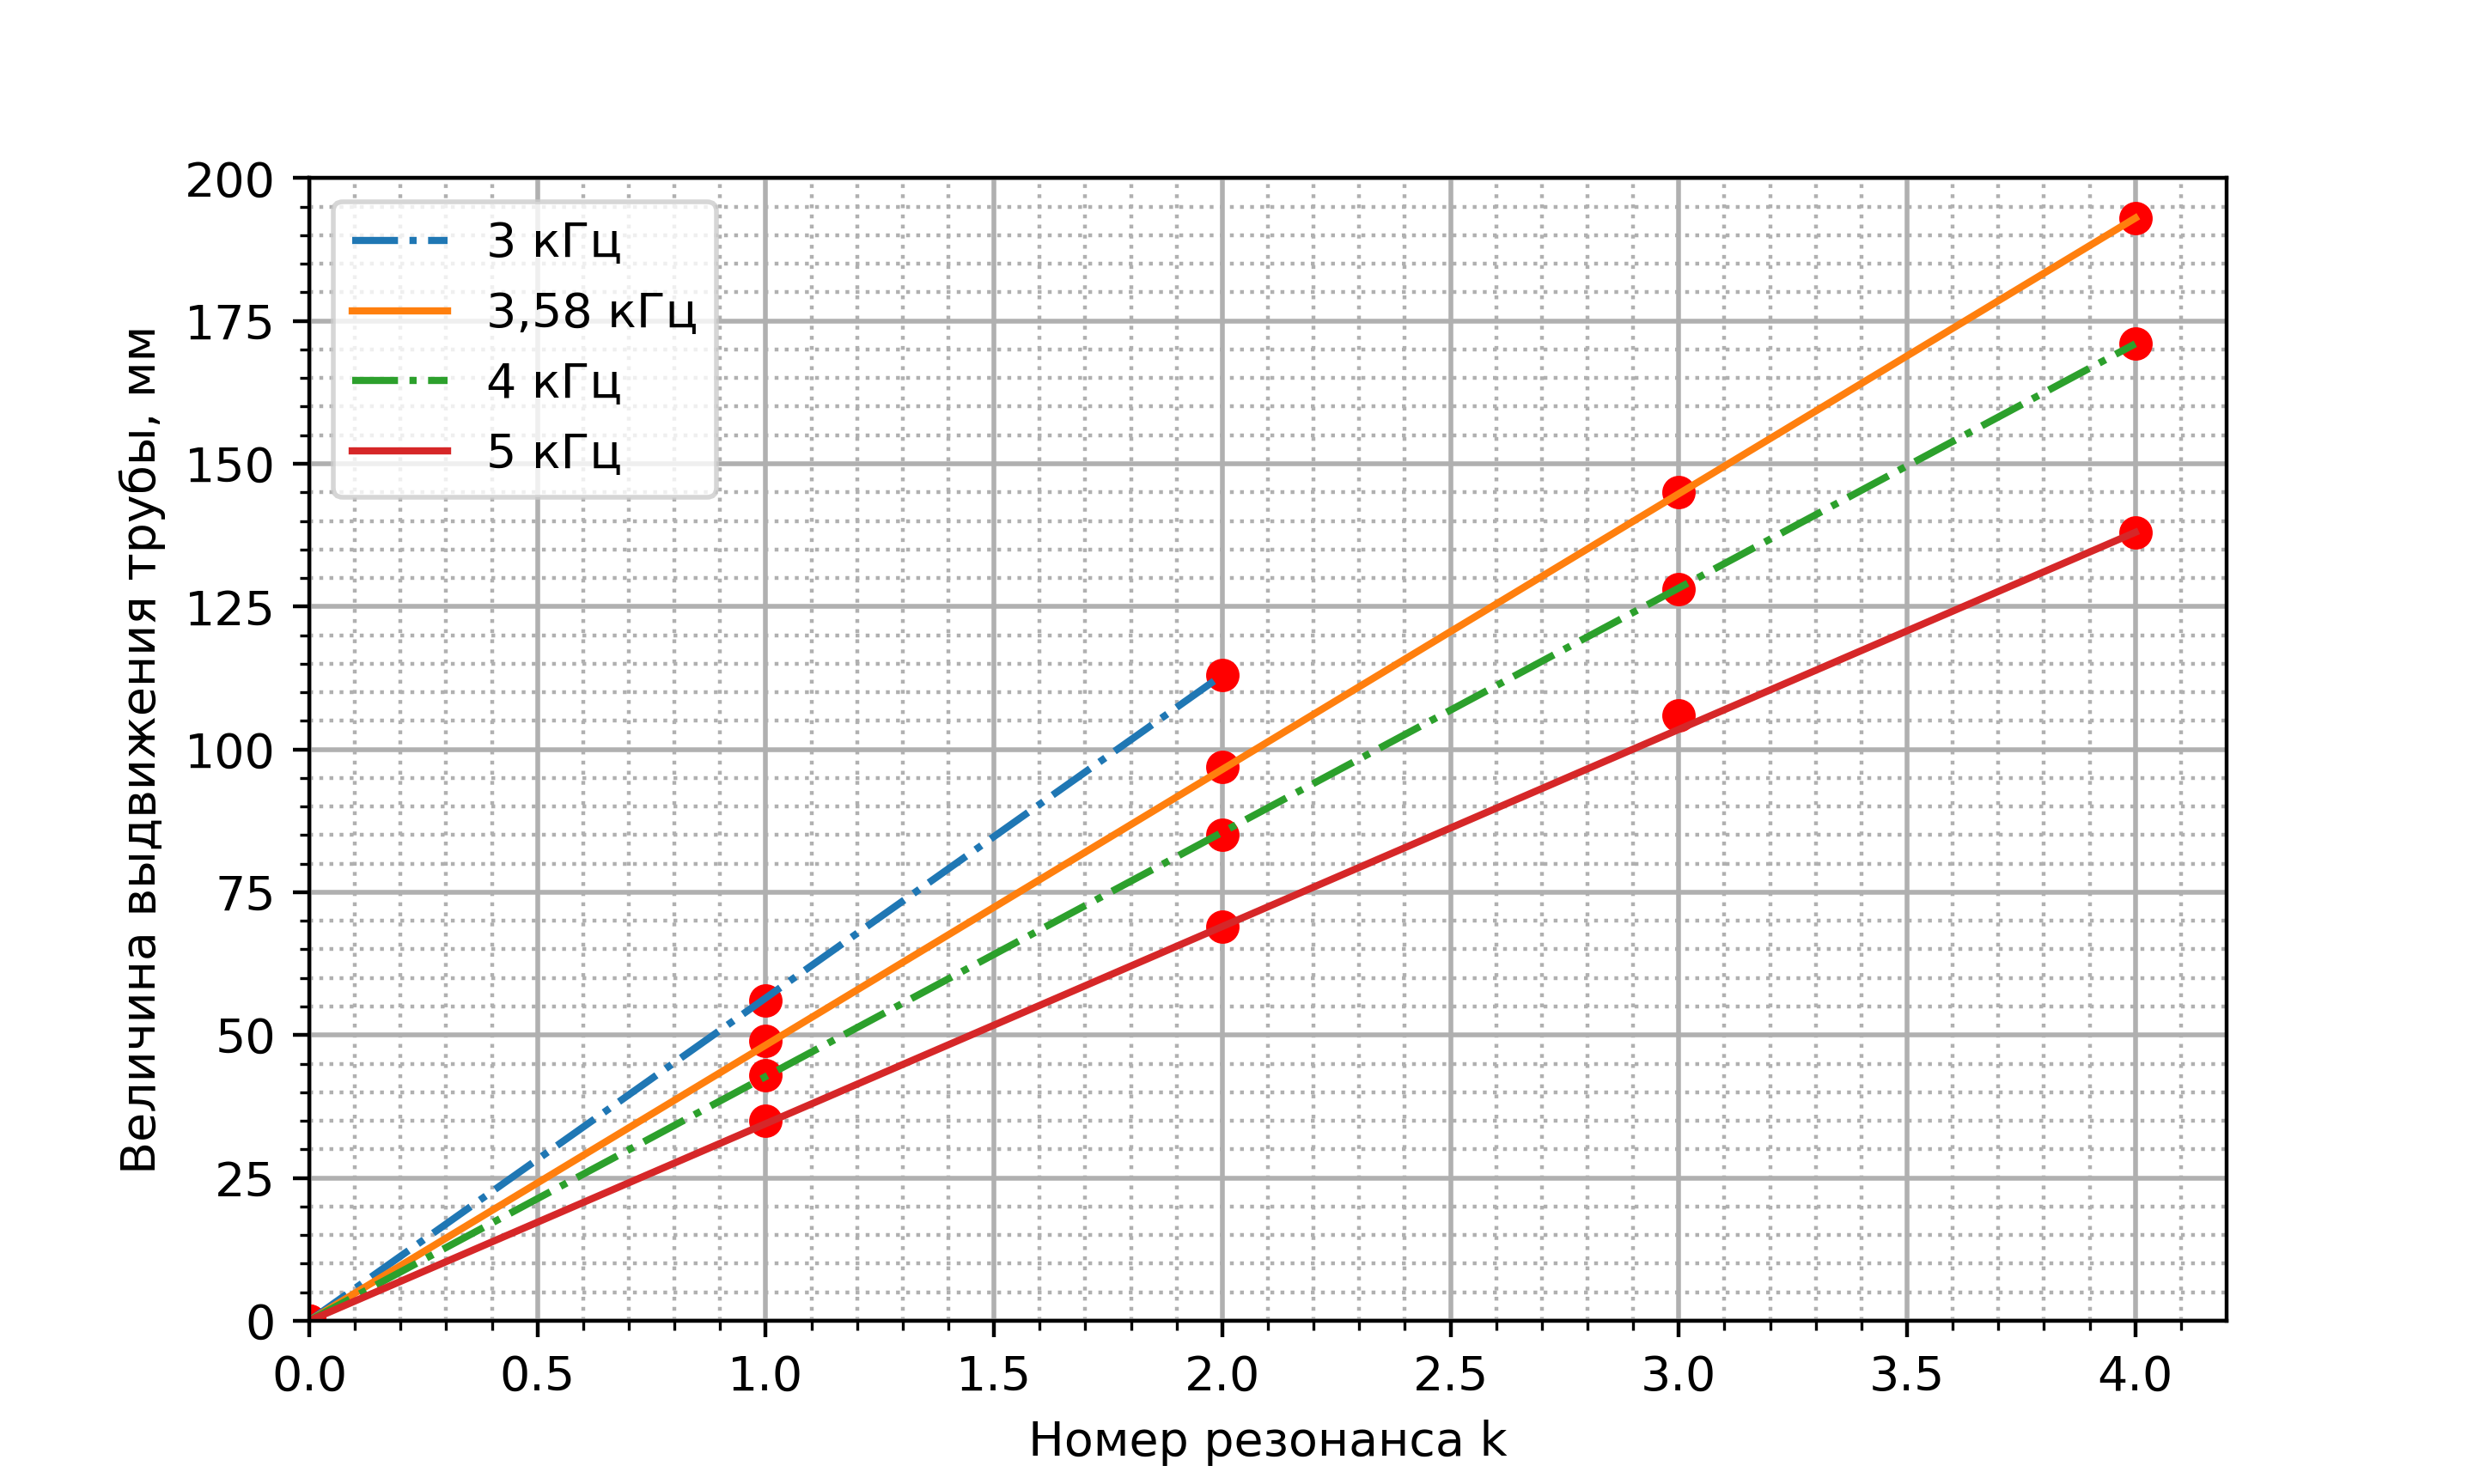
\includegraphics[width=\textwidth]{Gr1}
    \caption{}
    \end{figure}

Средние длины между резонансами - длины полуволн:

\begin{table}[H]
    \centering
    \caption{Таблица длин полуволн для воздуха.}
    \begin{tabular}{|l|l|l|l|l|}
    \hline
        Частота, кГц & 3.0  & 3.58  & 4.0  & 5.0 \\ \hline
        $\lambda/2$ , мм & 56.5 ± 0.2  & 48.2 ± 0.1  & 42.7 ± 0.1  & 34.7 ± 1.5 \\ \hline
    \end{tabular}
\end{table}

Используя $c = \lambda \nu$, найдем скорость звука в воздухе:

\begin{table}[H]
    \centering
    \caption{Таблица скоростей звука для воздуха.}
    \begin{tabular}{|l|l|l|l|l|}
    \hline
        Частота, кГц & 3.0  & 3.58  & 4.0  & 5.0 \\ \hline
        с, $\frac{м}{с}$ , мм & 339 ± 0.6  & 345 ± 0.4  & 342 ± 0.4 & 347 ± 0,1 \\ \hline
    \end{tabular}
\end{table}


    Табличное значение: $с = 340\frac{м}{с}$

\subsection{Измерение $ C_p/C_v $ для $CO_2$ при помощи установки с раздвижной трубой}

Закачаем в первую установку $CO_2$ и будем плавно менять длину трубы, записывая значения длин, на которых будет наблюдаться резонанс.


    \begin{table}[H]
    \centering
    \caption{\textbf{Результаты измерений для  $CO_2$}}
    \begin{tabular}{|l|l|l|l|l|l|}
    \hline
        Частота, кГц & 1 & 2,03 & 2,53 & 3,05 & 3,53 \\ \hline
        Удлинение 1, мм & 0 & 0 & 0 & 0 & 0 \\ \hline
        Удлинение 2, мм & 135 & 70 & 57 & 45 & 41 \\ \hline
        Удлинение 3, мм & ~ & 140 & 114 & 90 & 83 \\ \hline
        Удлинение 4, мм & ~ & ~ & 175 & 148 & 123 \\ \hline
        Удлинение 5, мм & ~ & ~ & ~ & 195 & 168 \\ \hline
    \end{tabular}
    \end{table}


    По полученным данным построим график:

    \begin{figure}[H]
    \centering
    \caption{График резонансов от удлинения трубы}
    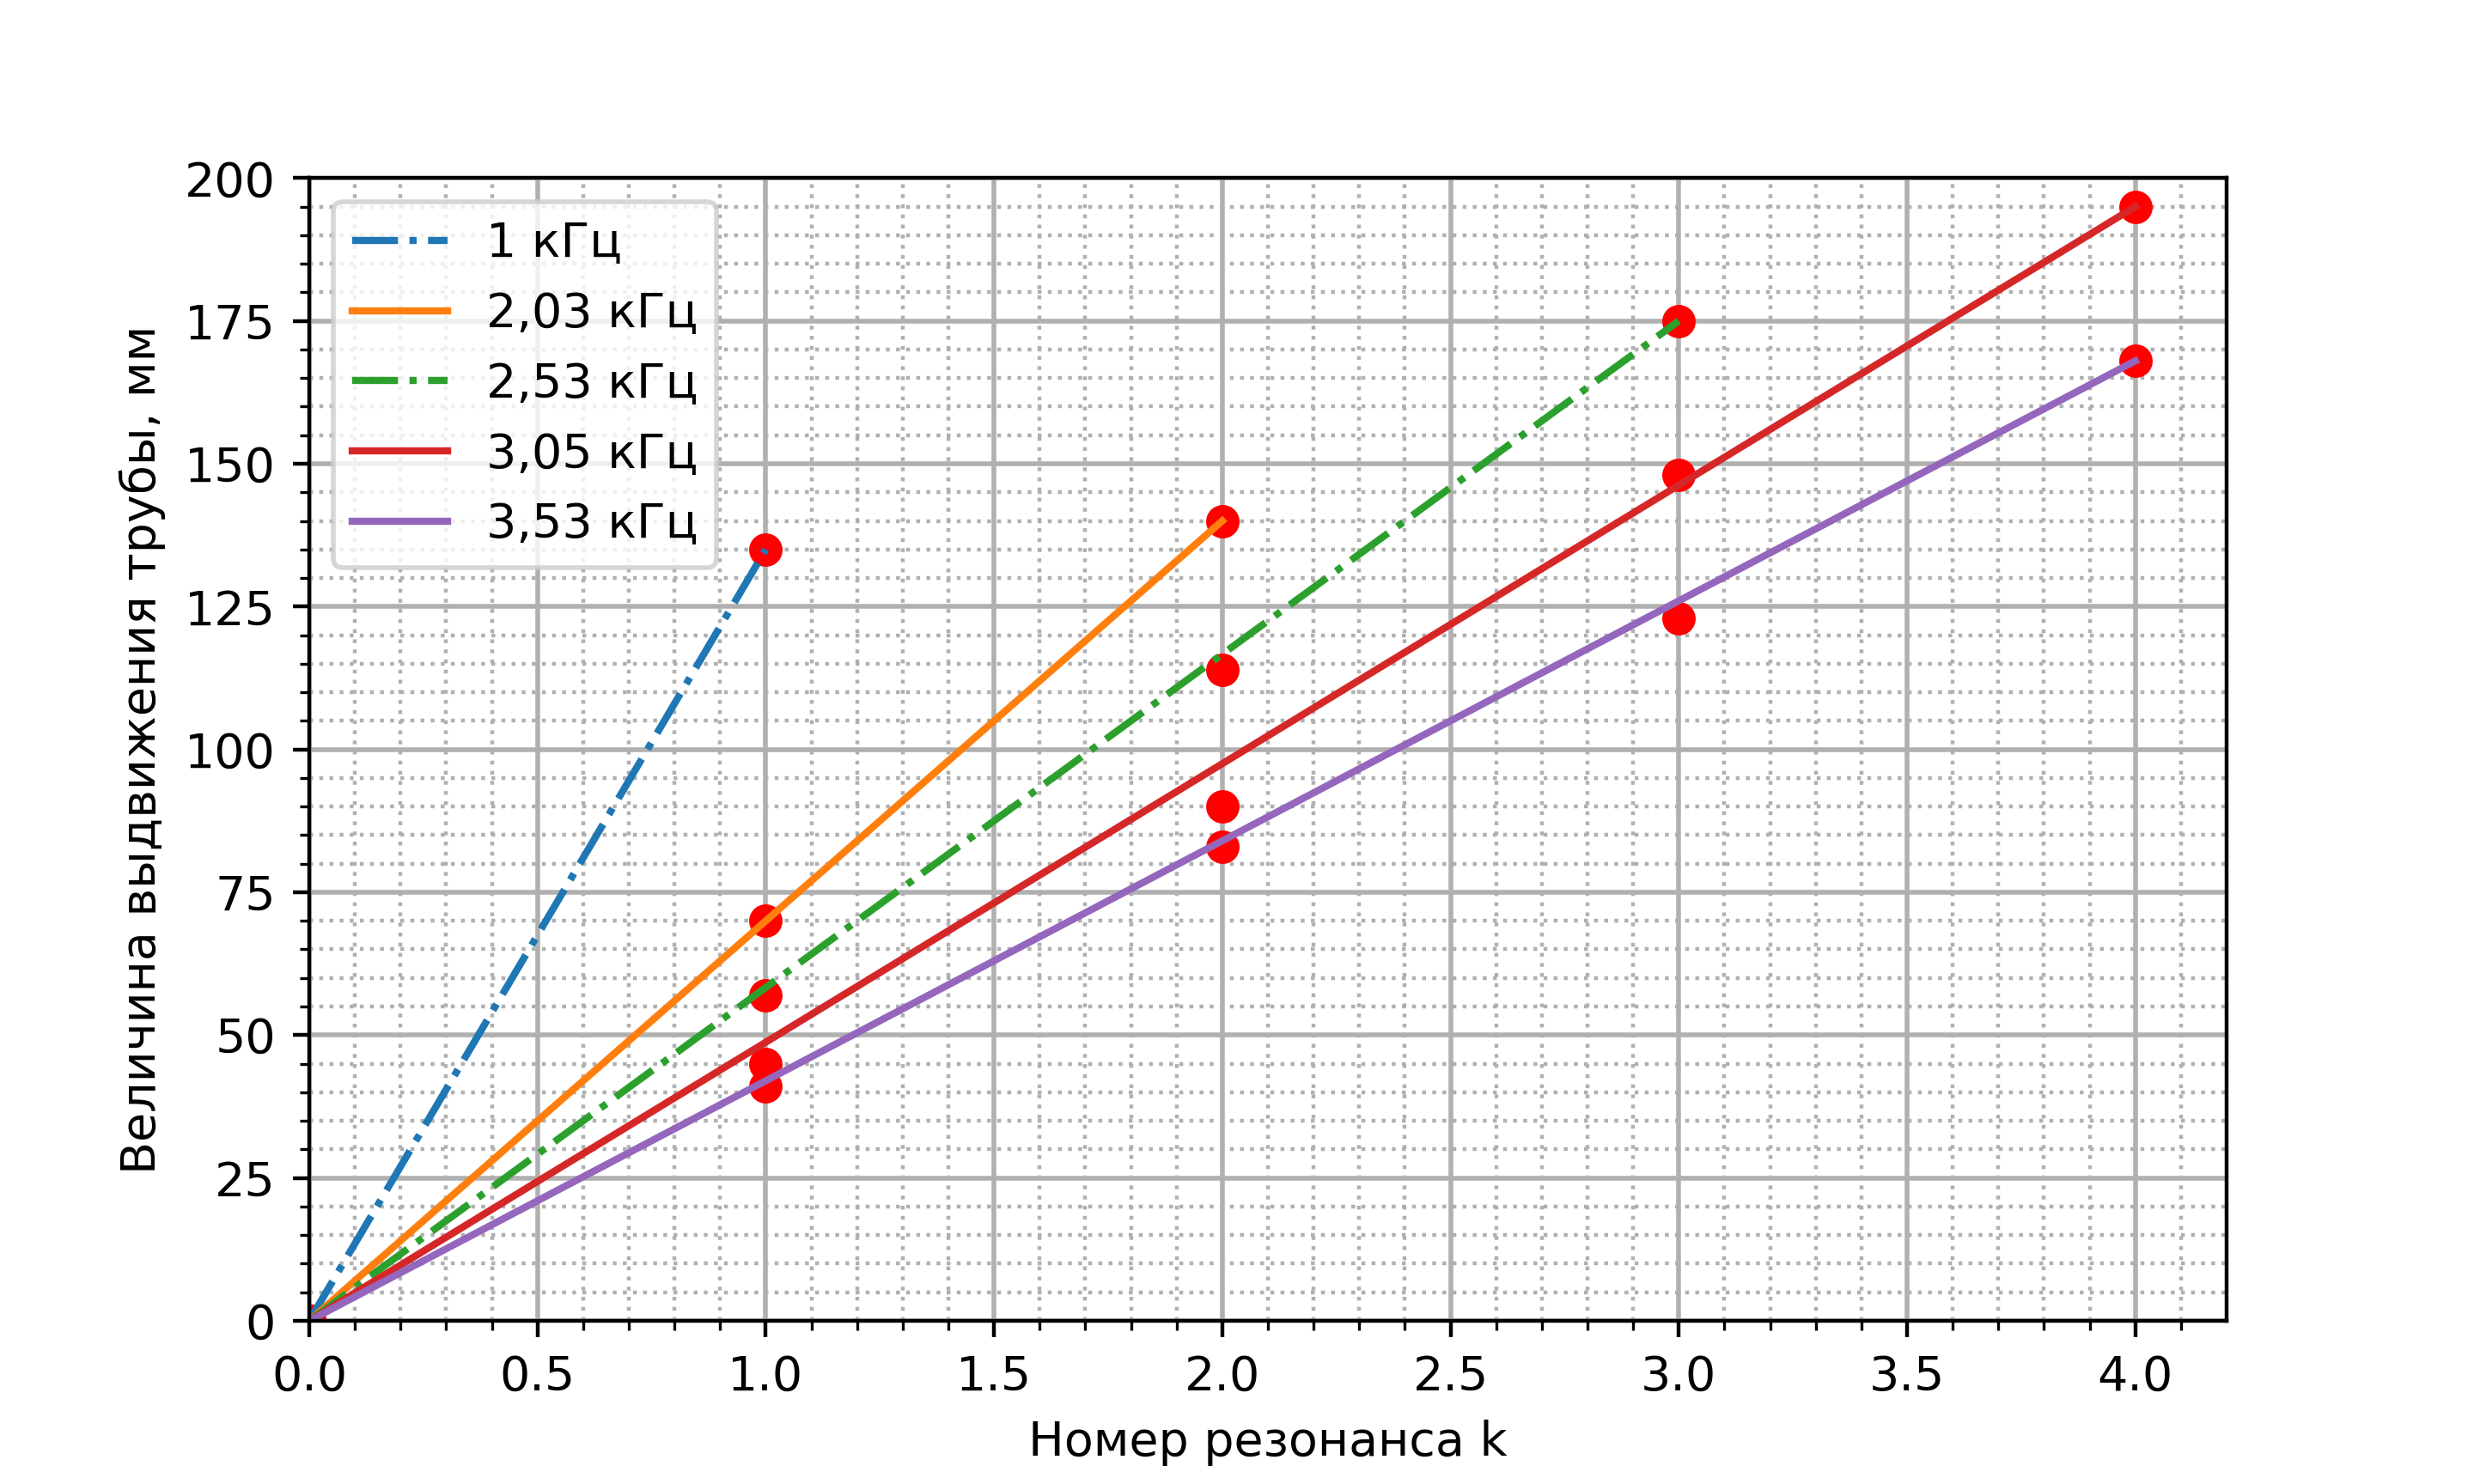
\includegraphics[width=\textwidth]{Gr2}
    \caption{}
    \end{figure}

Средние длины между резонансами - длины полуволн:

\begin{table}[H]
    \centering
    \caption{Таблица длин полуволн для $CO_2$.}
    \begin{tabular}{|l|l|l|l|l|l|}
    \hline
        Частота, кГц & 1  & 2  & 2,5  & 3,1 & 3,5 \\ \hline
        $\lambda/2$ , мм & 135 & 70  & 58.2 ± 0.5  & 49 ± 1 & 41,8 ± 0,3\\ \hline
    \end{tabular}
\end{table}

Используя $c = \lambda \nu$, найдем скорость звука в $CO_2$:

\begin{table}[H]
    \centering
    \caption{Таблица скоростей звука для $CO_2$.}
    \begin{tabular}{|l|l|l|l|l|l|}
    \hline
        Частота, кГц & 1  & 2  & 2,5  & 3,1 & 3,5 \\ \hline
        с, $\frac{м}{с}$ , мм & 270  & 280  & 291 ± 2 & 396 ±  3& 293 ± 1.1\\ \hline
    \end{tabular}
\end{table}


    Табличное значение: $с = 269\frac{м}{с}$

\subsection{Измерение $ C_p/C_v $ для воздуха при различных температурах}

Проведем измерения скорости звука в трубе постоянной длины. Плавно увеличивая частоту генератора, получим ряд последовательных резонансов. Повторим для разных температур:

\begin{table}[!ht]
    \centering
    \caption{\textbf{Результаты измерений}}
    \begin{tabular}{|l|l|l|l|l|}
    \hline
        T, K  & 297 & 308 & 315 & 323 \\ \hline
        резонанс 1, кГц  & 1,23 & 1,01 & 1,02 & 1,03 \\ \hline
        резонанс 2, кГц & 1,48 & 1,26 & 1,27 & 1,29 \\ \hline
        резонанс 3, кГц & 1,73 & 1,51 & 1,53 & 1,54 \\ \hline
        резонанс 4, кГц & 1,97 & 1,76 & 1,78 & 1,8 \\ \hline
        резонанс 5, кГц & 2,22 & 2,02 & 2,03 & ~ \\ \hline
    \end{tabular}
\end{table}

Построим график зависимости частоты от резонанса:

    \begin{figure}[H]
    \centering
    \caption{График зависимости $f_k(k)$ для воздуха}
    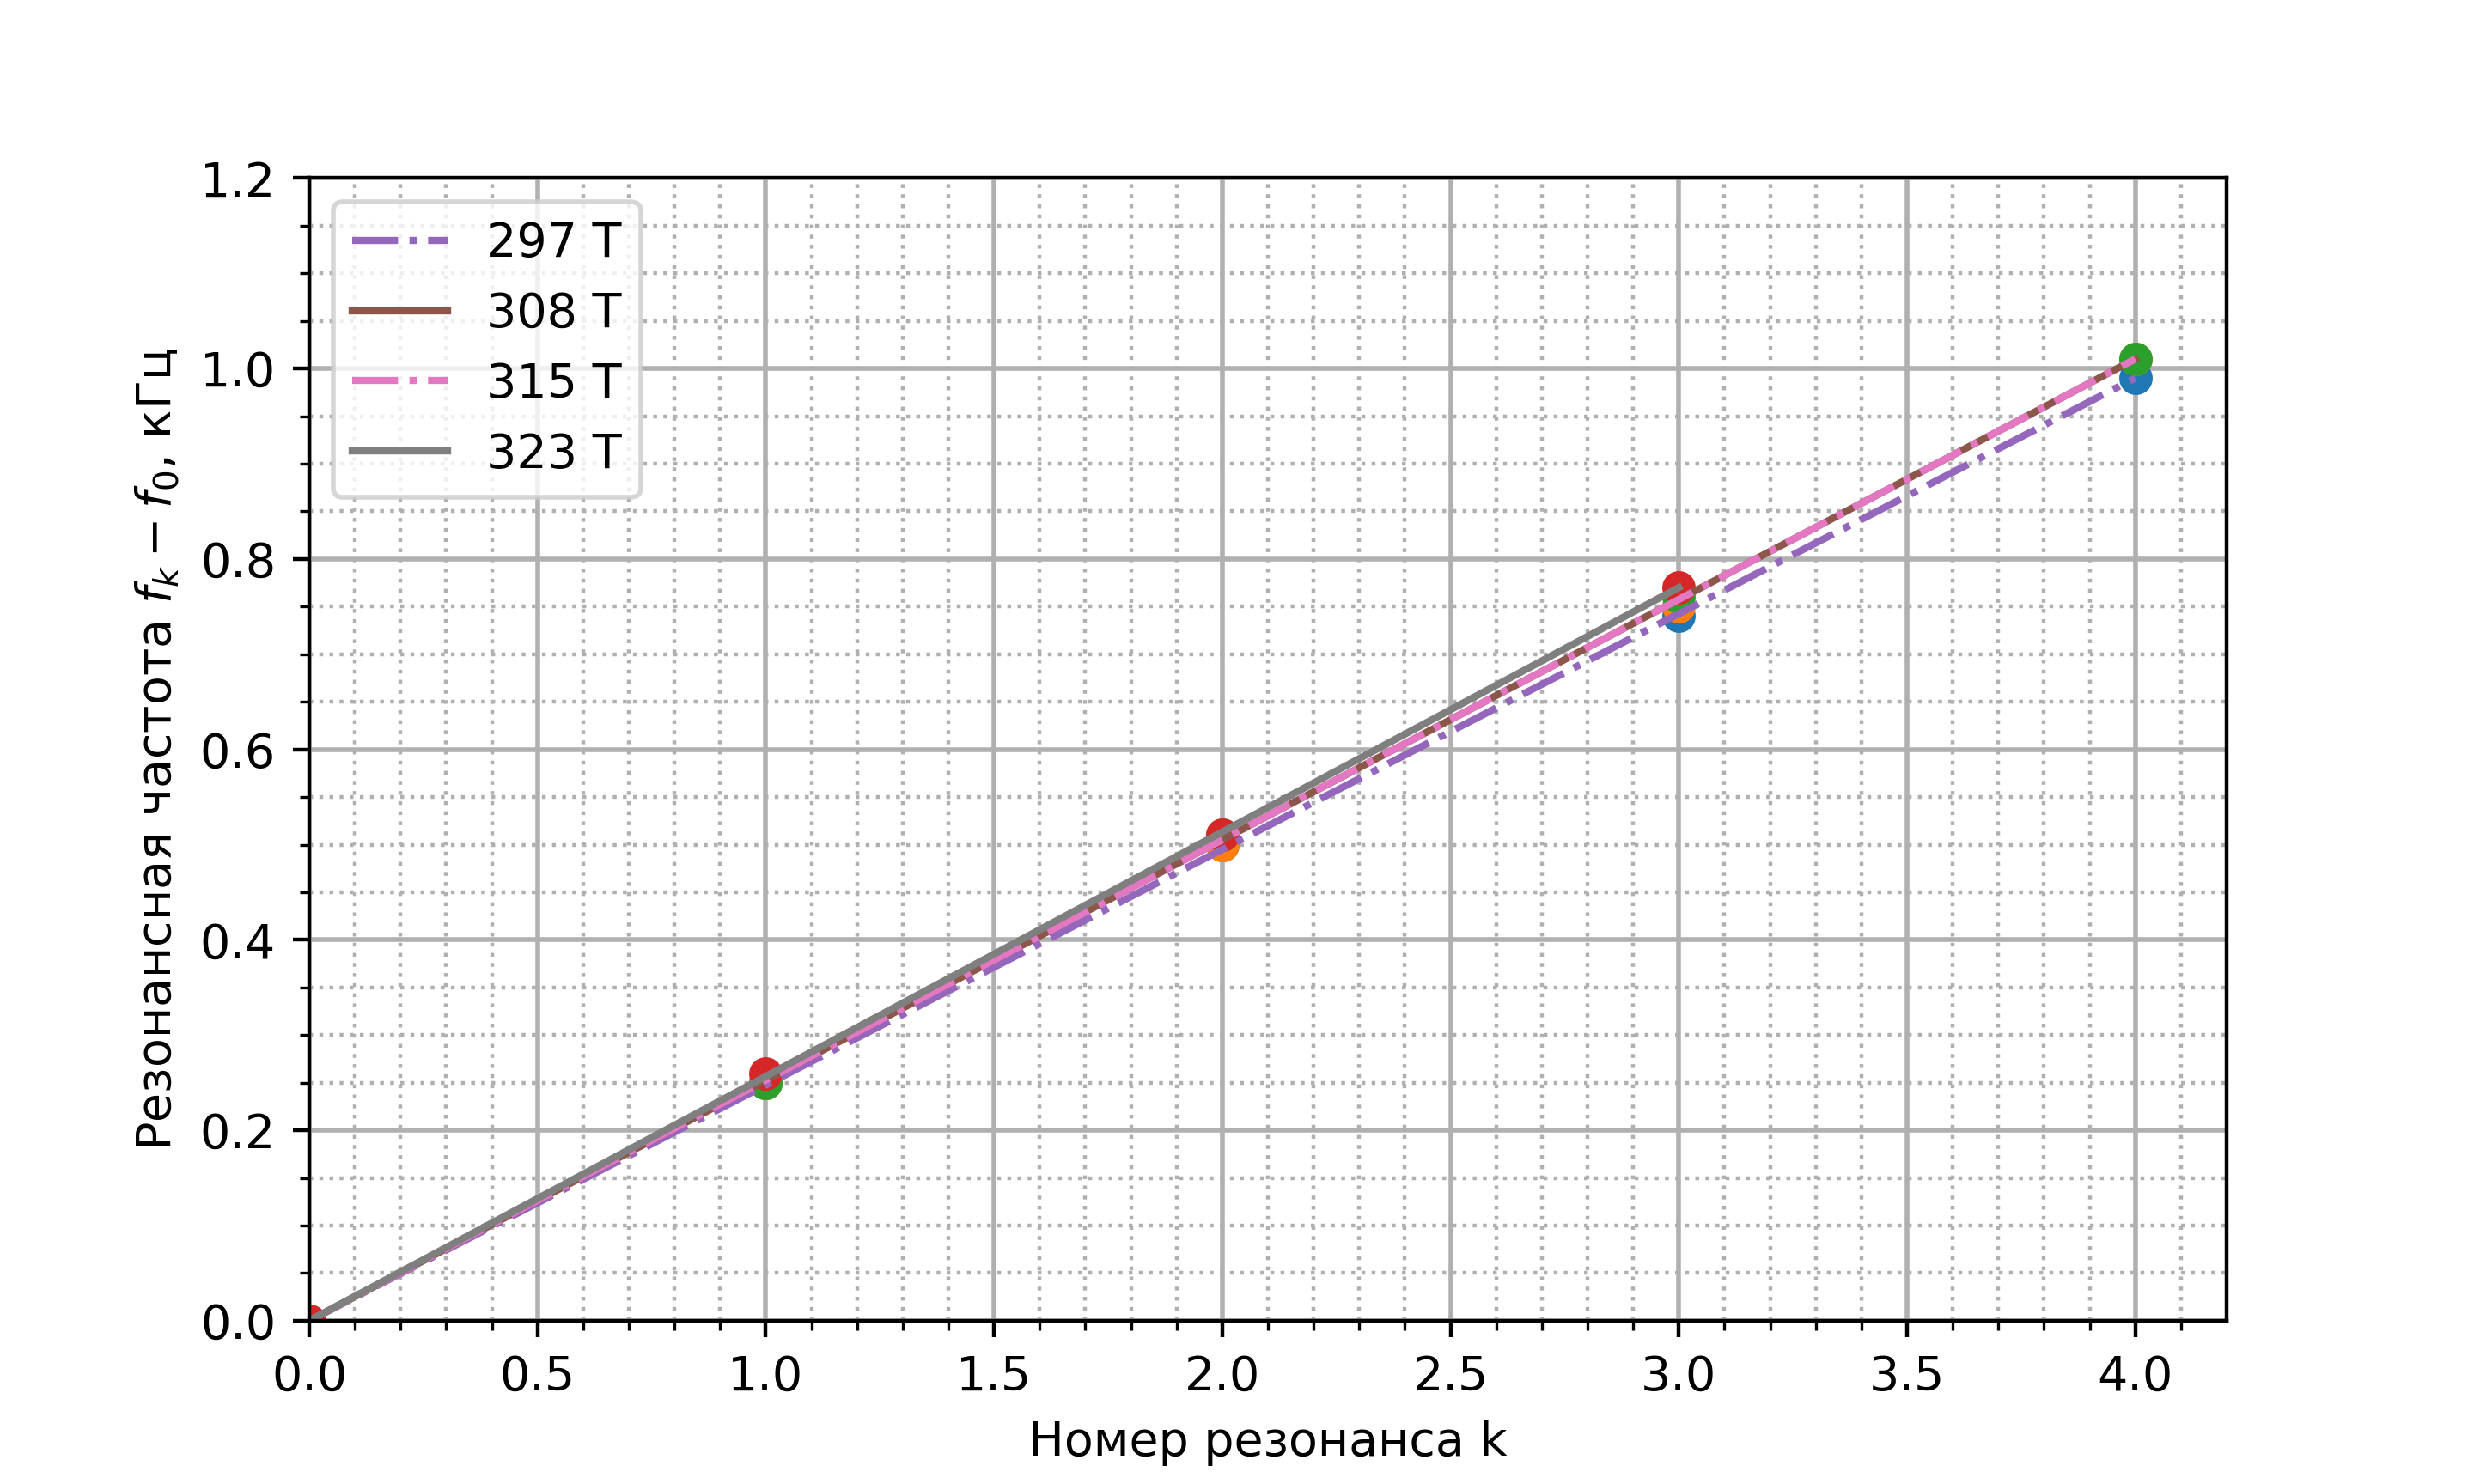
\includegraphics[width=\textwidth]{Gr3}
    \caption{}
    \end{figure}

Применим формулу, учитавая, что $L=700мм.$:
\[f_{k+l} - f_n = \frac{ck}{2L}\]

Вычислим скорости звука для каждого значения температуры: 

\begin{table}[!ht]
    \centering
    \begin{tabular}{|l|l|l|l|l|}
    \hline
        T, K  & 297 & 308 & 315 & 323 \\ \hline
        c, м/c & $345 ± 1 \cdot 10^{−3}$  & $352 ± 1 \cdot 10^{−3}$  & $354 ± 1 \cdot 10^{−3}$  & $358 ± 1 \cdot 10^{−3}$ \\ \hline
    \end{tabular}
\end{table} 

Мы видим, что результат хорошо согласуется с первым экспериментом и табличными значениями.
\subsection{Нахождение $\gamma = \frac{C_p}{C_v}$}

Воспользуемся формулой:

\[\gamma = \frac{\mu}{RT}c^2\]

Возьмём:
\[c=(343\pm 5,6)м/с\]
\[\mu_{возд} = 29 \frac{г}{моль}\]
\[T = 293 К\]

Тогда для воздуха: 
\[\gamma = 1,40 \pm 0,01\]

Табличное:
\[\gamma = 7/5 = 1,4\]

Для $CO_2$ при $с = (286 ± 13.4) м/c$:
\[\gamma = 1,47 \pm 0,01\]

Табличное:
\[\gamma = 1,3\]

\section{Вывод} 

В ходе лабораторной работы нами были вычислены скорости звука в воздухе и угликислом газе. При этом они довольно точно совпали с табличными.
Также стоит отметить, что в экспериментае наблюдался рост скорости звука с возрастанием температуры, что и предполагалось из теории.

С использованием полученных значений температуры
были получены значения коэффициента $\gamma$. Для воздуха он совпал с табличным, для углекислого газа же он отличается довольно сильно, это может быть связано с тем, что при измерениях в трубе находился углекислый газ с примесями, которые могли исказить результаты измерений.

\end{document}